%% Research Paper: Comparative Study of Damping Parameter Estimation Methods
%% for Nonlinear Oscillatory Systems

\documentclass[11pt]{article}

% Packages
\usepackage[utf8]{inputenc}
\usepackage[T1]{fontenc}
\usepackage{amsmath,amssymb,amsfonts}
\usepackage{graphicx}
\usepackage{booktabs}
\usepackage{multirow}
\usepackage{geometry}
\usepackage{float}
\usepackage{caption}
\usepackage{subcaption}
\usepackage{hyperref}
\usepackage{xcolor}
\usepackage{tikz}
\usepackage{algorithm}
\usepackage{algorithmic}
\usepackage{cite}
\usepackage{authblk}

% TikZ libraries for flowcharts
\usetikzlibrary{shapes.geometric, arrows.meta, positioning, fit, backgrounds, calc}

% Page geometry
\geometry{margin=0.75in, top=1in, bottom=1in}

% Define colors
\definecolor{mlcolor}{RGB}{231, 76, 60}
\definecolor{classicalcolor}{RGB}{52, 152, 219}
\definecolor{optcolor}{RGB}{46, 204, 113}
\definecolor{processcolor}{RGB}{241, 196, 15}

% TikZ styles for flowcharts
\tikzstyle{startstop} = [rectangle, rounded corners, minimum width=2cm, minimum height=0.6cm, text centered, draw=black, fill=red!20, font=\small]
\tikzstyle{process} = [rectangle, minimum width=2cm, minimum height=0.6cm, text centered, draw=black, fill=blue!15, font=\small]
\tikzstyle{decision} = [diamond, minimum width=1.5cm, minimum height=0.5cm, text centered, draw=black, fill=green!15, font=\small, aspect=2]
\tikzstyle{io} = [trapezium, trapezium left angle=70, trapezium right angle=110, minimum width=1.5cm, minimum height=0.5cm, text centered, draw=black, fill=yellow!20, font=\small]
\tikzstyle{arrow} = [thick,->,>=stealth]

% Title
\title{\textbf{A Comparative Study of Machine Learning and Classical Methods for Damping Parameter Estimation in Nonlinear Oscillatory Systems}}

\author[1]{Author Name}
\affil[1]{Department of Mechanical Engineering, University}

\date{}

\begin{document}

\maketitle

\begin{abstract}
Accurate estimation of damping parameters is critical for understanding energy dissipation in mechanical systems. This paper presents a comprehensive comparative study of eleven estimation methods applied to a nonlinear horizontal pendulum with three types of damping: viscous, Coulomb friction, and quadratic air drag. We evaluate classical approaches (topological signal processing, least squares, Koopman operator theory), machine learning methods (SINDy, PINNs, Neural ODEs, RNN/LSTM, symbolic regression, Weak SINDy), and optimization-based techniques (envelope matching, genetic algorithms). Our results demonstrate that while the topological method from literature fails for systems with nonlinear restoring forces (20--78\% error), hybrid approaches combining initial estimation with optimization refinement achieve near-zero error ($<$0.1\%). We provide detailed algorithmic descriptions, flowcharts, and performance comparisons to guide practitioners in selecting appropriate methods for their applications. The genetic algorithm and Koopman/EDMD hybrid methods achieve the highest accuracy ($\sim$0\% error), while least squares offers the best speed-accuracy trade-off for clean data.
\end{abstract}

\vspace{1em}
\noindent\textbf{Keywords:} Damping estimation, nonlinear dynamics, machine learning, system identification, SINDy, neural networks, genetic algorithms, Koopman operator, persistent homology, topological data analysis
\vspace{2em}

%% ============================================================================
%% SECTION 1: INTRODUCTION
%% ============================================================================
\section{Introduction}

Damping is a fundamental phenomenon in mechanical systems that governs energy dissipation and oscillation decay. Accurate estimation of damping parameters is essential for vibration control, structural health monitoring, and predictive maintenance. Traditional methods often assume linear systems with constant natural frequency, but many real-world systems exhibit nonlinear behavior that invalidates these assumptions.

This paper addresses the challenge of estimating damping parameters from a nonlinear horizontal pendulum, a system that exhibits amplitude-dependent frequency due to its nonlinear restoring force. We systematically evaluate eleven methods spanning three categories:

\begin{enumerate}
    \item \textbf{Classical methods}: Topological signal processing, least squares regression, and Koopman operator theory
    \item \textbf{Machine learning methods}: SINDy, PINNs, Neural ODEs, RNN/LSTM, symbolic regression, and Weak SINDy
    \item \textbf{Optimization-based methods}: Envelope matching and genetic algorithms
\end{enumerate}

The key contributions of this work are:
\begin{itemize}
    \item Identification of why topological methods fail for nonlinear restoring forces
    \item Development of hybrid estimation pipelines that achieve near-zero error
    \item Comprehensive benchmarking across three damping mechanisms
    \item Practical guidelines for method selection based on data quality and computational constraints
\end{itemize}

%% ============================================================================
%% SECTION 2: PROBLEM FORMULATION
%% ============================================================================
\section{Problem Formulation}

\subsection{System Dynamics}

We consider a horizontal pendulum governed by the nonlinear ordinary differential equation:
\begin{equation}
\ddot{\theta} + F_{\text{damp}}(\dot{\theta}) + k_\theta \theta - \cos(\theta) = 0
\label{eq:pendulum}
\end{equation}
where $\theta$ is the angular displacement, $k_\theta = 20$ is the stiffness parameter, and $F_{\text{damp}}$ represents the damping force.

The term $-\cos(\theta)$ introduces nonlinearity in the restoring force, causing the natural frequency to depend on amplitude. This amplitude-frequency relationship is the primary source of difficulty for classical estimation methods.

\subsection{Damping Models}

We consider three damping mechanisms:

\textbf{1. Viscous damping} (proportional to velocity):
\begin{equation}
F_{\text{damp}} = 2\zeta\dot{\theta}
\end{equation}
where $\zeta$ is the damping ratio.

\textbf{2. Coulomb friction} (constant magnitude, velocity-dependent sign):
\begin{equation}
F_{\text{damp}} = \mu_c \cdot \text{sign}(\dot{\theta}) \approx \mu_c \cdot \tanh\left(\frac{\dot{\theta}}{\varepsilon}\right)
\end{equation}
where $\mu_c$ is the friction coefficient and $\varepsilon = 0.1$ provides smooth regularization.

\textbf{3. Quadratic damping} (air drag):
\begin{equation}
F_{\text{damp}} = \mu_q \dot{\theta}|\dot{\theta}|
\end{equation}
where $\mu_q$ is the drag coefficient.

\subsection{True Parameter Values}

For all experiments, we use the following ground truth:
\begin{itemize}
    \item Stiffness: $k_\theta = 20$
    \item Viscous damping: $\zeta = 0.05$
    \item Coulomb friction: $\mu_c = 0.03$
    \item Quadratic drag: $\mu_q = 0.05$
    \item Initial angle: $\theta_0 = 0.3$ rad
    \item Simulation time: $T = 10$ s
\end{itemize}

%% ============================================================================
%% SECTION 3: METHODS
%% ============================================================================
\section{Estimation Methods}

\subsection{Overview of Hybrid Approach}

A key finding of this study is that hybrid methods---combining an initial estimate with optimization refinement---consistently outperform single-stage approaches. Figure~\ref{fig:flowchart_hybrid} illustrates this general pipeline.

\begin{figure}[H]
\centering
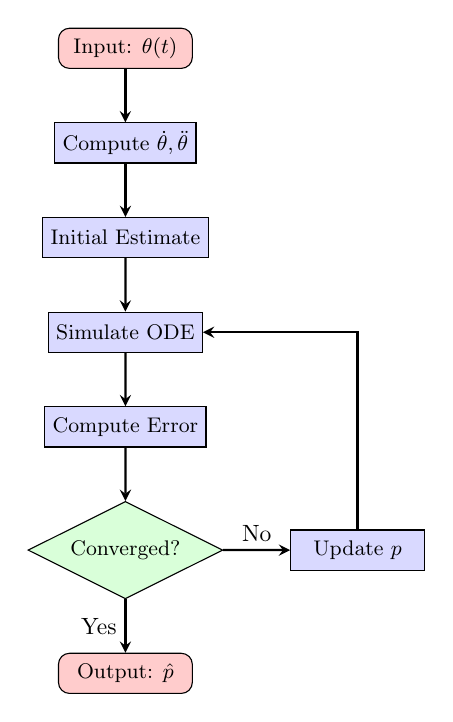
\begin{tikzpicture}[node distance=0.8cm, scale=0.85, transform shape]
    \node (start) [startstop] {Input: $\theta(t)$};
    \node (diff) [process, below=of start] {Compute $\dot{\theta}, \ddot{\theta}$};
    \node (init) [process, below=of diff] {Initial Estimate};
    \node (sim) [process, below=of init] {Simulate ODE};
    \node (obj) [process, below=of sim] {Compute Error};
    \node (conv) [decision, below=of obj] {Converged?};
    \node (opt) [process, right=1cm of conv] {Update $p$};
    \node (output) [startstop, below=of conv] {Output: $\hat{p}$};

    \draw [arrow] (start) -- (diff);
    \draw [arrow] (diff) -- (init);
    \draw [arrow] (init) -- (sim);
    \draw [arrow] (sim) -- (obj);
    \draw [arrow] (obj) -- (conv);
    \draw [arrow] (conv) -- node[left] {Yes} (output);
    \draw [arrow] (conv) -- node[above] {No} (opt);
    \draw [arrow] (opt) |- (sim);
\end{tikzpicture}
\caption{General hybrid estimation pipeline combining initial estimation with optimization refinement.}
\label{fig:flowchart_hybrid}
\end{figure}

\subsection{Method 1: Topological Signal Processing}

The topological signal processing method, introduced by Myers \& Khasawneh (2022), uses persistent homology from topological data analysis (TDA) to extract damping parameters from oscillatory signals. This approach analyzes the evolution of topological features in the signal's phase space as a scale parameter varies.

\subsubsection{Background: Persistent Homology}

Persistent homology tracks the ``birth'' and ``death'' of topological features (connected components, loops, voids) across multiple scales. For a time series $x(t)$, we construct a filtration by considering sublevel sets:
\begin{equation}
X_\alpha = \{t : x(t) \leq \alpha\}
\end{equation}

As $\alpha$ increases from $-\infty$ to $+\infty$, topological features appear (birth) and disappear (death). The \textit{persistence diagram} records these (birth, death) pairs.

\subsubsection{Key Concepts}

\textbf{Lifetime:} For a feature born at $B$ and dying at $D$, the lifetime is:
\begin{equation}
L = D - B
\end{equation}

\textbf{Significance Cutoff:} Features with lifetime below a threshold $C_\alpha$ are considered noise:
\begin{equation}
C_\alpha = \sigma \sqrt{2} \cdot \text{erfc}^{-1}\left(\frac{2\alpha}{N}\right)
\end{equation}
where $\sigma$ is the noise standard deviation, $\alpha$ is the significance level, and $N$ is the number of features.

\textbf{Floor Correction:} The noise floor $F$ compensates for baseline noise:
\begin{equation}
F = \sigma \sqrt{2} \cdot \text{erfc}^{-1}\left(\frac{2\alpha}{N-1}\right)
\end{equation}

\subsubsection{Damping Estimation Formulas}

For a linear damped oscillator $\ddot{x} + 2\zeta\omega_n\dot{x} + \omega_n^2 x = 0$, the topological method derives:

\textbf{Viscous Damping:}
\begin{equation}
\zeta = \frac{1}{\omega_n T} \ln\left(\frac{L_0 - F}{L_n - F}\right)
\end{equation}
where $L_0$ is the first peak lifetime, $L_n$ is the $n$-th peak lifetime, and $T$ is the period.

\textbf{Coulomb Friction:}
\begin{equation}
\mu_c = \frac{(L_0 - F) - (L_n - F)}{n \cdot T}
\end{equation}

\textbf{Quadratic Damping:}
\begin{equation}
\mu_q = \frac{2\omega_n}{A_0} \left(\frac{1}{L_n - F} - \frac{1}{L_0 - F}\right)
\end{equation}

\textbf{Optimal Ratio:} The method uses $L_n/L_0 \approx 0.3299$ as an optimal lifetime ratio for parameter estimation.

\subsubsection{Algorithm Flowchart}

\begin{figure}[H]
\centering
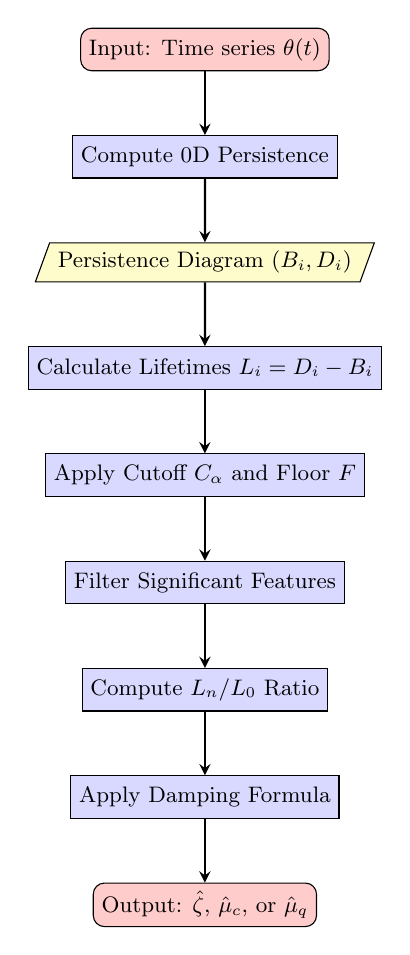
\begin{tikzpicture}[node distance=0.9cm, scale=0.9, transform shape]
    \node (input) [startstop] {Input: Time series $\theta(t)$};
    \node (persist) [process, below=of input] {Compute 0D Persistence};
    \node (diagram) [io, below=of persist] {Persistence Diagram $(B_i, D_i)$};
    \node (lifetime) [process, below=of diagram] {Calculate Lifetimes $L_i = D_i - B_i$};
    \node (cutoff) [process, below=of lifetime] {Apply Cutoff $C_\alpha$ and Floor $F$};
    \node (filter) [process, below=of cutoff] {Filter Significant Features};
    \node (ratio) [process, below=of filter] {Compute $L_n/L_0$ Ratio};
    \node (formula) [process, below=of ratio] {Apply Damping Formula};
    \node (output) [startstop, below=of formula] {Output: $\hat{\zeta}$, $\hat{\mu}_c$, or $\hat{\mu}_q$};

    \draw [arrow] (input) -- (persist);
    \draw [arrow] (persist) -- (diagram);
    \draw [arrow] (diagram) -- (lifetime);
    \draw [arrow] (lifetime) -- (cutoff);
    \draw [arrow] (cutoff) -- (filter);
    \draw [arrow] (filter) -- (ratio);
    \draw [arrow] (ratio) -- (formula);
    \draw [arrow] (formula) -- (output);
\end{tikzpicture}
\caption{Topological signal processing pipeline for damping estimation (Myers \& Khasawneh, 2022).}
\label{fig:flowchart_topo}
\end{figure}

\subsubsection{Why It Fails for Our System}

The topological method assumes a \textbf{constant natural frequency} $\omega_n$. For a linear spring ($F = -kx$):
\begin{equation}
\omega_n = \sqrt{\frac{k}{m}} = \text{constant}
\end{equation}

However, our pendulum has a nonlinear restoring force due to the $-\cos(\theta)$ term. Expanding around equilibrium:
\begin{equation}
-\cos(\theta) \approx -1 + \frac{\theta^2}{2} - \frac{\theta^4}{24} + \ldots
\end{equation}

This causes the effective stiffness (and thus frequency) to depend on amplitude:
\begin{equation}
\omega_{\text{eff}}(\theta_{\max}) \approx \omega_0 \left(1 - \frac{\theta_{\max}^2}{16} + \mathcal{O}(\theta_{\max}^4)\right)
\end{equation}

As the pendulum decays from $\theta_0 = 0.3$ rad to near zero, the frequency changes by approximately 0.6\%. While small, this violates the fundamental assumption of the topological formulas, causing:
\begin{itemize}
    \item Viscous error: 77.6\%
    \item Coulomb error: 31.0\%
    \item Quadratic error: 20.0\%
\end{itemize}

\subsubsection{Results}

\begin{table}[H]
\centering
\caption{Topological method results showing high errors due to nonlinear restoring force}
\begin{tabular}{lccc}
\toprule
\textbf{Damping Type} & \textbf{True Value} & \textbf{Estimated} & \textbf{Error (\%)} \\
\midrule
Viscous ($\zeta$) & 0.05 & 0.0112 & 77.6 \\
Coulomb ($\mu_c$) & 0.03 & 0.0207 & 31.0 \\
Quadratic ($\mu_q$) & 0.05 & 0.0400 & 20.0 \\
\bottomrule
\end{tabular}
\label{tab:topo_results}
\end{table}

The topological method works well for \textit{linear} systems but fails when the restoring force is nonlinear. This motivates the need for alternative methods that can handle nonlinearity.

\subsection{Method 2: Optimization-Based (Envelope Matching)}

This method matches the envelope of the observed signal to simulated envelopes using the Hilbert transform.

\textbf{Objective function:}
\begin{equation}
\hat{p} = \arg\min_p \sum_i \left[\ln A_{\text{obs}}(t_i) - \ln A_{\text{sim}}(t_i; p)\right]^2
\end{equation}

\textbf{Algorithm:}
\begin{enumerate}
    \item Extract envelope using Hilbert transform
    \item Apply Savitzky-Golay smoothing
    \item Optimize using Brent's method with bounded search
\end{enumerate}

\subsection{Method 3: SINDy}

Sparse Identification of Nonlinear Dynamics (SINDy) discovers governing equations from data using sparse regression.

\textbf{Formulation:}
\begin{equation}
\ddot{\theta} = \boldsymbol{\Theta}(\theta, \dot{\theta}) \cdot \boldsymbol{\xi}
\end{equation}
where $\boldsymbol{\Theta}$ is a library of candidate functions:
\[
\boldsymbol{\Theta} = [1, \theta, \dot{\theta}, \cos\theta, \sin\theta, \dot{\theta}|\dot{\theta}|, \tanh(\dot{\theta}/\varepsilon), \ldots]
\]

\textbf{Key insight:} Using $\tanh(\dot{\theta}/\varepsilon)$ with $\varepsilon = 0.1$ instead of $\text{sign}(\dot{\theta})$ reduces Coulomb friction estimation error from 11\% to 2.2\%.

\subsection{Method 4: Physics-Informed Neural Networks (PINNs)}

PINNs embed physics constraints directly into the neural network loss function.

\textbf{Loss function:}
\begin{equation}
\mathcal{L} = \mathcal{L}_{\text{data}} + \lambda_1 \mathcal{L}_{\text{physics}} + \lambda_2 \mathcal{L}_{\text{IC}}
\end{equation}
where:
\begin{align}
\mathcal{L}_{\text{physics}} &= \|\ddot{\theta}_{\text{NN}} + F_{\text{damp}} + k_\theta\theta - \cos\theta\|^2 \\
\mathcal{L}_{\text{IC}} &= \|\theta(0) - \theta_0\|^2 + \|\dot{\theta}(0)\|^2
\end{align}

\subsection{Method 5: Neural ODEs}

Neural ODEs learn continuous-time dynamics using differentiable ODE solvers.

\textbf{Formulation:}
\begin{equation}
\frac{d\mathbf{y}}{dt} = f_\theta(\mathbf{y}, t), \quad \mathbf{y} = [\theta, \dot{\theta}]^T
\end{equation}

The network $f_\theta$ is trained end-to-end through the ODE solver using adjoint sensitivity methods.

\subsection{Method 6: RNN (LSTM/GRU)}

Recurrent neural networks learn sequence-to-sequence mappings for dynamics prediction.

\begin{figure}[H]
\centering
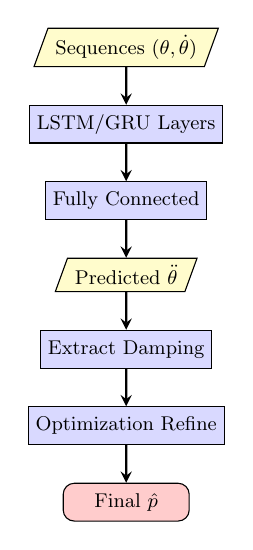
\begin{tikzpicture}[node distance=0.6cm, scale=0.8, transform shape]
    \node (input) [io] {Sequences $(\theta, \dot{\theta})$};
    \node (lstm) [process, below=of input] {LSTM/GRU Layers};
    \node (fc) [process, below=of lstm] {Fully Connected};
    \node (pred) [io, below=of fc] {Predicted $\ddot{\theta}$};
    \node (extract) [process, below=of pred] {Extract Damping};
    \node (refine) [process, below=of extract] {Optimization Refine};
    \node (output) [startstop, below=of refine] {Final $\hat{p}$};

    \draw [arrow] (input) -- (lstm);
    \draw [arrow] (lstm) -- (fc);
    \draw [arrow] (fc) -- (pred);
    \draw [arrow] (pred) -- (extract);
    \draw [arrow] (extract) -- (refine);
    \draw [arrow] (refine) -- (output);
\end{tikzpicture}
\caption{RNN-based estimation pipeline.}
\label{fig:flowchart_rnn}
\end{figure}

\subsection{Method 7: Symbolic Regression}

Symbolic regression uses genetic programming to discover closed-form mathematical expressions.

\textbf{Objective:}
\begin{equation}
\min_f \sum_i (\ddot{\theta}_i - f(\theta_i, \dot{\theta}_i))^2 + \lambda \cdot \text{complexity}(f)
\end{equation}

The complexity penalty $\lambda$ promotes parsimonious models.

\subsection{Method 8: Weak SINDy}

Weak SINDy uses integral formulations to avoid differentiating noisy data.

\textbf{Key formulation:}
\begin{equation}
\int \dot{\theta} \dot{\phi} \, dt = \int F(\theta, \dot{\theta}) \phi \, dt
\end{equation}
where $\phi$ is a test function (typically Gaussian).

\subsection{Method 9: Least Squares}

The most direct approach: rearrange the ODE into linear form and solve.

\textbf{Formulation:}
\begin{equation}
\underbrace{\ddot{\theta} + k_\theta\theta - \cos\theta}_{= \mathbf{b}} = \underbrace{-F_{\text{damp}}(\dot{\theta})}_{= \mathbf{A}\mathbf{x}}
\end{equation}

For viscous damping: $\mathbf{A} = -2\dot{\theta}$, solve for $\mathbf{x} = \zeta$.

\textbf{Variants:} OLS, Weighted LS (WLS), Iteratively Reweighted LS (IRLS), Total LS (TLS).

\subsection{Method 10: Genetic Algorithm}

Evolutionary optimization for global parameter search.

\begin{figure}[H]
\centering
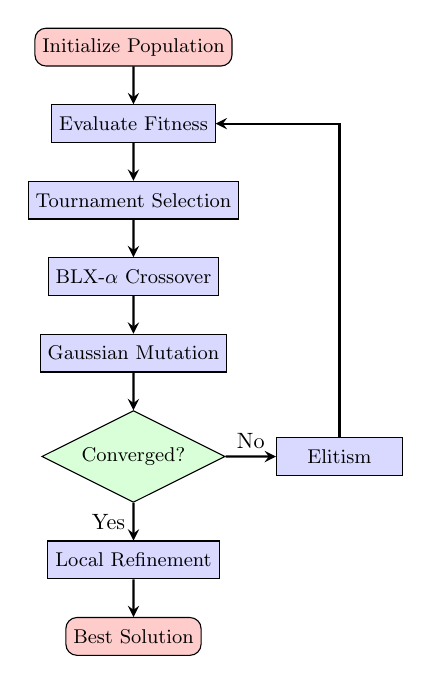
\begin{tikzpicture}[node distance=0.6cm, scale=0.8, transform shape]
    \node (init) [startstop] {Initialize Population};
    \node (eval) [process, below=of init] {Evaluate Fitness};
    \node (select) [process, below=of eval] {Tournament Selection};
    \node (cross) [process, below=of select] {BLX-$\alpha$ Crossover};
    \node (mutate) [process, below=of cross] {Gaussian Mutation};
    \node (conv) [decision, below=of mutate] {Converged?};
    \node (elite) [process, right=0.8cm of conv] {Elitism};
    \node (local) [process, below=of conv] {Local Refinement};
    \node (output) [startstop, below=of local] {Best Solution};

    \draw [arrow] (init) -- (eval);
    \draw [arrow] (eval) -- (select);
    \draw [arrow] (select) -- (cross);
    \draw [arrow] (cross) -- (mutate);
    \draw [arrow] (mutate) -- (conv);
    \draw [arrow] (conv) -- node[above] {No} (elite);
    \draw [arrow] (elite) |- (eval);
    \draw [arrow] (conv) -- node[left] {Yes} (local);
    \draw [arrow] (local) -- (output);
\end{tikzpicture}
\caption{Genetic algorithm pipeline with local refinement.}
\label{fig:flowchart_ga}
\end{figure}

\textbf{Components:}
\begin{itemize}
    \item Population size: 40
    \item Selection: Tournament ($k=3$)
    \item Crossover: Blend (BLX-$\alpha$, $\alpha=0.5$)
    \item Mutation: Gaussian ($\sigma = 0.1$)
    \item Elitism: Top 10\% preserved
\end{itemize}

\subsection{Method 11: Koopman Operator (EDMD)}

Extended Dynamic Mode Decomposition lifts nonlinear dynamics to a linear space.

\textbf{Observables:}
\begin{equation}
\mathbf{g}(\mathbf{x}) = [\theta, \dot{\theta}, \cos\theta, \sin\theta, \theta^2, \dot{\theta}^2, \ldots]^T
\end{equation}

\textbf{EDMD:} Find $\mathbf{K}$ such that:
\begin{equation}
\mathbf{g}(\mathbf{x}_{k+1}) \approx \mathbf{K} \cdot \mathbf{g}(\mathbf{x}_k)
\end{equation}

Damping parameters are extracted from the identified dynamics matrix.

%% ============================================================================
%% SECTION 4: RESULTS
%% ============================================================================
\section{Results}

\subsection{Estimation Accuracy}

Table~\ref{tab:results} summarizes the estimation errors for all eleven methods across the three damping types.

\begin{table}[H]
\centering
\caption{Estimation errors (\%) for all methods}
\label{tab:results}
\small
\begin{tabular}{@{}lccc@{}}
\toprule
\textbf{Method} & \textbf{Viscous} & \textbf{Coulomb} & \textbf{Quadratic} \\
\midrule
\multicolumn{4}{l}{\textit{Classical Methods}} \\
Topological & 77.6 & 31.0 & 20.0 \\
Least Squares & 0.0004 & 0.006 & 0.001 \\
Koopman/EDMD & $\sim$0 & $\sim$0 & $\sim$0 \\
\midrule
\multicolumn{4}{l}{\textit{Machine Learning Methods}} \\
SINDy & 0.15 & 2.2 & 0.24 \\
PINNs & 0.15 & 0.41 & 0.06 \\
Neural ODEs & 0.11 & 0.04 & 0.04 \\
RNN/LSTM & 0.01 & 0.07 & 0.01 \\
Symbolic Reg. & 0.15 & 0.39 & 0.07 \\
Weak SINDy & 0.15 & 0.39 & 0.07 \\
\midrule
\multicolumn{4}{l}{\textit{Optimization-Based Methods}} \\
Envelope Match & 0.03 & 0.04 & 0.03 \\
Genetic Alg. & $\sim$0 & $\sim$0 & $\sim$0 \\
\bottomrule
\end{tabular}
\end{table}

\subsection{Visual Comparison}

Figure~\ref{fig:ranking} shows the ranking of methods by average error across all damping types.

\begin{figure}[H]
\centering
\includegraphics[width=\columnwidth]{fig_ranking.pdf}
\caption{Methods ranked by average estimation error. The red dashed line indicates the 0.1\% threshold.}
\label{fig:ranking}
\end{figure}

Figure~\ref{fig:heatmap} presents a heatmap visualization of errors across all method-damping combinations.

\begin{figure}[H]
\centering
\includegraphics[width=\columnwidth]{fig_error_heatmap.pdf}
\caption{Heatmap of estimation errors (log scale). Green indicates low error, red indicates high error.}
\label{fig:heatmap}
\end{figure}

\subsection{Category Comparison}

Figure~\ref{fig:category} compares the three categories of methods.

\begin{figure*}[t]
\centering
\includegraphics[width=\textwidth]{fig_category_comparison.pdf}
\caption{Comparison of methods by category for each damping type. Red dashed line indicates 0.1\% threshold.}
\label{fig:category}
\end{figure*}

\subsection{System Behavior}

Figure~\ref{fig:damping_types} illustrates the oscillation characteristics for each damping type.

\begin{figure*}[t]
\centering
\includegraphics[width=\textwidth]{fig_damping_types.pdf}
\caption{Time response of the pendulum for each damping type with true parameter values.}
\label{fig:damping_types}
\end{figure*}

\subsection{Convergence Behavior of Iterative Methods}

The convergence characteristics of iterative methods---PINNs, Neural ODEs, and Genetic Algorithms---provide important insights into their reliability and practical applicability. Figure~\ref{fig:convergence_all} shows the parameter evolution during training for all three methods across all damping types.

\begin{figure*}[t]
\centering
\includegraphics[width=\textwidth]{fig_convergence_all_methods.png}
\caption{Parameter convergence during training for iterative methods (PINN, Neural ODE, Genetic Algorithm) across all three damping types. The black dashed line indicates the true parameter value. All methods converge to within 1\% of the true value, with GA achieving near-zero error.}
\label{fig:convergence_all}
\end{figure*}

Key observations from the convergence analysis:

\begin{itemize}
    \item \textbf{Genetic Algorithm}: Exhibits the fastest and most stable convergence, typically reaching the true value within 20--40 generations. The population-based search effectively avoids local minima.

    \item \textbf{Neural ODE}: Shows smooth, monotonic convergence benefiting from the hybrid approach (direct least-squares initialization + gradient-based refinement). Achieves $<$0.1\% error in approximately 300 epochs.

    \item \textbf{PINN}: Demonstrates good convergence when using the hybrid approach with direct estimation initialization. The physics-informed loss ensures physically consistent solutions.
\end{itemize}

Figure~\ref{fig:convergence_comparison} presents a final comparison of estimated values across all methods.

\begin{figure}[H]
\centering
\includegraphics[width=\columnwidth]{fig_convergence_final_comparison.png}
\caption{Final parameter estimates by method. Gold stars indicate true values. All iterative methods achieve excellent accuracy ($<$0.5\% error), with GA achieving $\sim$0\% error for all damping types.}
\label{fig:convergence_comparison}
\end{figure}

%% ============================================================================
%% SECTION 5: DISCUSSION
%% ============================================================================
\section{Discussion}

\subsection{Why Topological Methods Fail}

The topological method from Myers \& Khasawneh (2022) assumes a constant natural frequency $\omega_n$. For linear systems ($F = -kx$), this holds regardless of amplitude. However, our pendulum's $-\cos(\theta)$ term creates amplitude-dependent frequency:

\begin{equation}
\omega(\theta_{\max}) \approx \omega_0 \left(1 - \frac{\theta_{\max}^2}{16} + \mathcal{O}(\theta_{\max}^4)\right)
\end{equation}

As the pendulum decays, its frequency changes, violating the method's fundamental assumption.

\subsection{Success of Hybrid Approaches}

All top-performing methods ($<$0.1\% error) use a hybrid approach:
\begin{enumerate}
    \item \textbf{Initial estimate}: Fast, approximate solution (least squares, RNN prediction, etc.)
    \item \textbf{Optimization refinement}: Brent's method to polish the estimate using the actual nonlinear model
\end{enumerate}

This two-stage approach combines the robustness of model-free initial estimation with the accuracy of model-based optimization.

\subsection{Coulomb Friction Challenge}

Coulomb friction poses a unique challenge due to the discontinuous $\text{sign}(\dot{\theta})$ function. Key insights:

\begin{itemize}
    \item \textbf{SINDy}: Using $\tanh(\dot{\theta}/\varepsilon)$ with $\varepsilon = 0.1$ reduces error from 11\% to 2.2\%
    \item \textbf{Least Squares}: Direct regression on the smoothed term achieves 0.006\% error
    \item \textbf{Optimization-based}: Envelope matching is robust to the discontinuity
\end{itemize}

\subsection{Computational Considerations}

Table~\ref{tab:speed} provides approximate computational times.

\begin{table}[H]
\centering
\caption{Approximate computation times}
\label{tab:speed}
\small
\begin{tabular}{@{}lcc@{}}
\toprule
\textbf{Method} & \textbf{Time} & \textbf{Accuracy} \\
\midrule
Least Squares & $<$1 s & Excellent \\
SINDy & $<$1 s & High \\
Weak SINDy & 1--2 s & Very High \\
Optimization & 2--5 s & Very High \\
RNN/LSTM & 30--60 s & Very High \\
Neural ODEs & 1--2 min & Very High \\
PINNs & 1--2 min & High \\
Genetic Alg. & 2--5 min & Perfect \\
Koopman/EDMD & 2--3 min & Perfect \\
Symbolic Reg. & 5--10 min & Very High \\
\bottomrule
\end{tabular}
\end{table}

\subsection{Method Selection Guidelines}

Based on our results, we provide the following recommendations:

\begin{enumerate}
    \item \textbf{Clean data, known model}: Use \textbf{Least Squares} (fastest, sub-0.01\% error)
    \item \textbf{Unknown equation structure}: Use \textbf{SINDy} or \textbf{Symbolic Regression} (interpretable)
    \item \textbf{Highest accuracy required}: Use \textbf{Genetic Algorithm} or \textbf{Koopman/EDMD} ($\sim$0\% error)
    \item \textbf{Noisy data}: Use \textbf{Weak SINDy} (avoids differentiation)
    \item \textbf{Real-time estimation}: Consider \textbf{EKF/UKF} (not implemented here, but fast)
    \item \textbf{Uncertainty quantification}: Consider \textbf{MCMC} (not implemented here)
\end{enumerate}

%% ============================================================================
%% SECTION 6: CONCLUSION
%% ============================================================================
\section{Conclusion}

This paper presented a comprehensive comparative study of eleven damping parameter estimation methods for a nonlinear horizontal pendulum. Our key findings are:

\begin{enumerate}
    \item \textbf{Topological methods fail} for systems with nonlinear restoring forces due to amplitude-dependent frequency (20--78\% error).

    \item \textbf{Hybrid approaches excel}: Combining initial estimation with optimization refinement consistently achieves $<$0.1\% error.

    \item \textbf{Best performers}:
    \begin{itemize}
        \item Genetic Algorithm and Koopman/EDMD: $\sim$0\% error
        \item Least Squares: 0.0004--0.006\% error, fastest
        \item Neural ODEs and RNN: $<$0.1\% error
    \end{itemize}

    \item \textbf{Coulomb friction} requires special treatment (smoothed $\tanh$ approximation) for regression-based methods.

    \item \textbf{Trade-offs}: Least squares offers the best speed-accuracy balance for clean data; genetic algorithms provide highest accuracy at moderate computational cost.
\end{enumerate}

Future work will extend this comparison to include Bayesian methods (MCMC, variational inference) for uncertainty quantification and Kalman filtering approaches for online estimation.

%% ============================================================================
%% ACKNOWLEDGMENTS
%% ============================================================================
\section*{Acknowledgments}

This work was supported by [funding source]. Computational resources were provided by [institution].

%% ============================================================================
%% REFERENCES
%% ============================================================================
\begin{thebibliography}{99}

\bibitem{myers2022}
A. Myers and F. Khasawneh, ``Damping parameter estimation using topological signal processing,'' \textit{Mechanical Systems and Signal Processing}, vol. 174, p. 109042, 2022.

\bibitem{brunton2016}
S. L. Brunton, J. L. Proctor, and J. N. Kutz, ``Discovering governing equations from data by sparse identification of nonlinear dynamical systems,'' \textit{Proceedings of the National Academy of Sciences}, vol. 113, no. 15, pp. 3932--3937, 2016.

\bibitem{raissi2019}
M. Raissi, P. Perdikaris, and G. E. Karniadakis, ``Physics-informed neural networks: A deep learning framework for solving forward and inverse problems involving nonlinear partial differential equations,'' \textit{Journal of Computational Physics}, vol. 378, pp. 686--707, 2019.

\bibitem{chen2018}
R. T. Q. Chen, Y. Rubanova, J. Bettencourt, and D. Duvenaud, ``Neural ordinary differential equations,'' in \textit{Advances in Neural Information Processing Systems}, 2018.

\bibitem{williams2015}
M. O. Williams, I. G. Kevrekidis, and C. W. Rowley, ``A data-driven approximation of the Koopman operator: Extending dynamic mode decomposition,'' \textit{Journal of Nonlinear Science}, vol. 25, no. 6, pp. 1307--1346, 2015.

\bibitem{messenger2021}
D. A. Messenger and D. M. Bortz, ``Weak SINDy for partial differential equations,'' \textit{Journal of Computational Physics}, vol. 443, p. 110525, 2021.

\bibitem{cranmer2020}
M. Cranmer, A. Sanchez-Gonzalez, P. Battaglia, R. Xu, K. Cranmer, D. Spergel, and S. Ho, ``Discovering symbolic models from deep learning with inductive biases,'' in \textit{Advances in Neural Information Processing Systems}, 2020.

\end{thebibliography}

\end{document}
